\chapter{Пружинка}
\label{ch:chap4}
Параметры системы:
$$
M = 24, \tab k = 112
$$
Даны уравнения пружинного маятника:
$$
F_{ela} = -kx, \tab F = ma = m\ddot{x}
$$
Входом считается $F_{ext}(t)$ - некая внешняя соосно направленная сила, а $x(t)$ - выход. 
Запишем второй закон Ньютона, чтобы объединить уравнения:
$$
    F = F_{ela} + F_{ext} = m\ddot{x}
$$

\section{Передаточная функция}
Перейдем в операторную форму Лапласа:
$$
 -kX + F_{ext} = ms^2X
$$
$$
W(s) = \frac{1}{ms^2 + k}
$$
По отсутствию компоненты $s$ в знаменателе видно, что это - \textit{консервативное звено}, его общий вид:
$$
W(S) = \frac{K}{T^2s^2 + 1}
$$ Тогда в нашем случае $K = \frac{1}{mk} \approx 4\cdot 10^{-4}$ и $T = \sqrt{\frac{1}{k}} \approx 0.09$
\section{Временные  характеристики}
$$
\begin{aligned}
    y_{i.r.}(t) = \mathcal{L}^{-1}\{\frac{K}{T^2s^2 + 1}\} = \mathcal{L}^{-1}\{\frac{K}{T^2(s^2 + \frac{1}{T^2})}\} = \mathcal{L}^{-1}\{\frac{K \frac{1}{T}}{\frac{1}{T}T^2(s^2 + \frac{1}{T^2})}\} = \\
    \frac{K}{T} sin(\frac{1}{T}t)
\end{aligned}
$$
$$
    \begin{aligned}
        y_{s.r.}(t) = \mathcal{L}^{-1}\{\frac{K}{s(T^2s^2 + 1)}\} = \mathcal{L}^{-1}\{\frac{K}{s} - \frac{T^2s}{T^2s^2 + 1}\} = \mathcal{L}^{-1}\{\frac{K}{s} - \frac{Ks}{s^2 + \frac{1}{T^2}}\} = \\
        K - K\cdot cos(\frac{1}{T}t)
    \end{aligned}
$$
\newpage
\begin{figure}[ht]
  \centering
  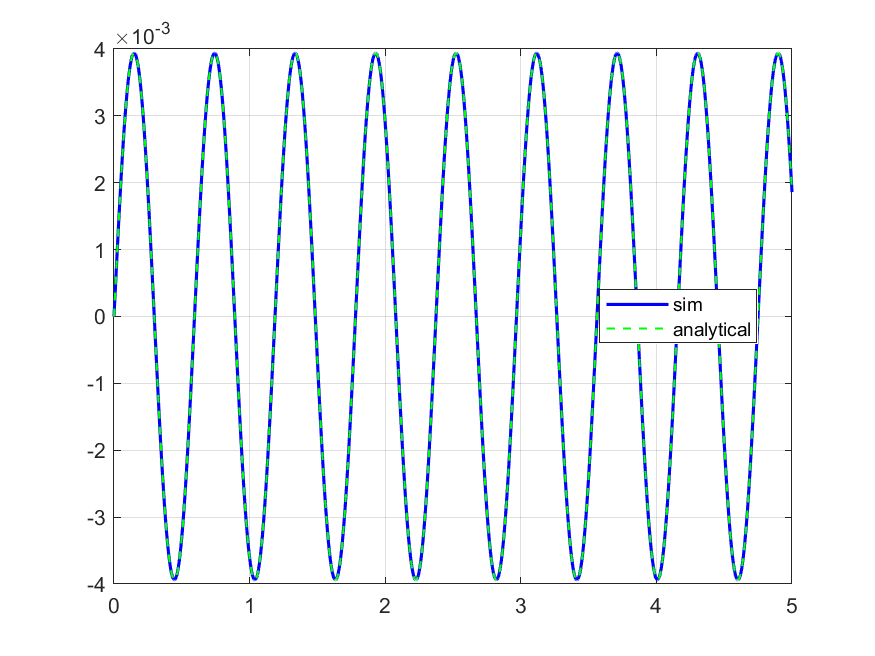
\includegraphics[width=0.8\textwidth]{impulse_responce4.png}
  \caption{Воздействие - \textrm{impulse responce}}
\end{figure}

\begin{figure}[ht]
    \centering
    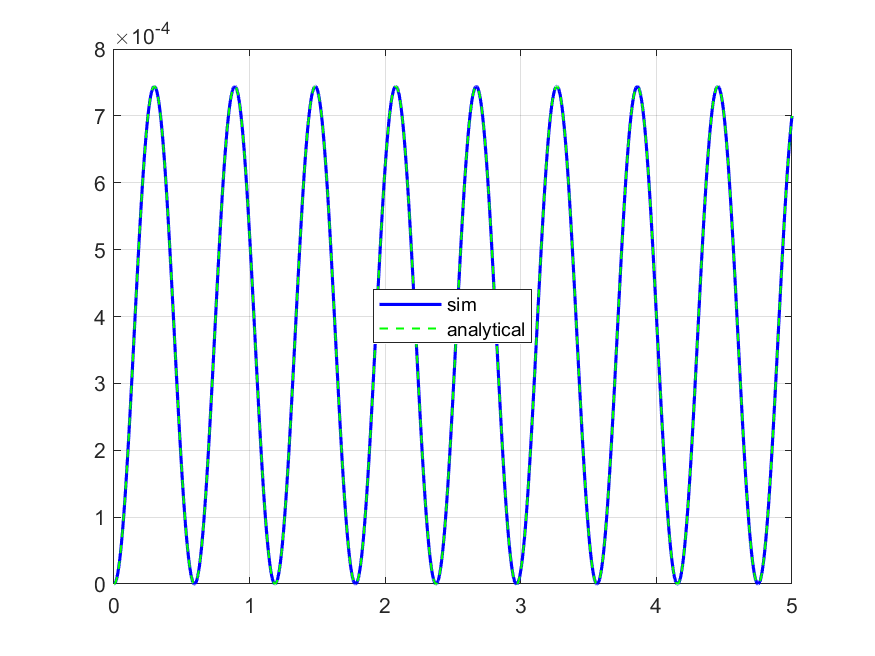
\includegraphics[width=0.8\textwidth]{step_responce4.png}
    \caption{Воздействие - \textrm{step responce}}
  \end{figure}
\newpage
\section{Частотные характеристики}
$$
W(j\omega) =  \frac{K}{T^2(j\omega)^2 + 1} = \frac{K}{1  - T^2\omega^2} + 0
$$
Амплитудно-частотная характеристика:
$$
A(\omega) = \sqrt{P^2 + Q^2} = \sqrt{(\frac{K}{1  - T^2\omega^2})^2 + 0^2} =  \frac{K}{|1  - T^2\omega^2|}
$$
Логарифмическая-Амплитудно-частотная характеристика:
$$
L(\omega) = 20lg(A) = 20lg(K) - 20lg(|1  - T^2\omega^2|)
$$
Фазовая-частотная характеристика:
$$
\phi(\omega) = -atan2(0, \frac{K}{1  - T^2\omega^2})
$$
\newpage
\begin{figure}[ht]
  \centering
  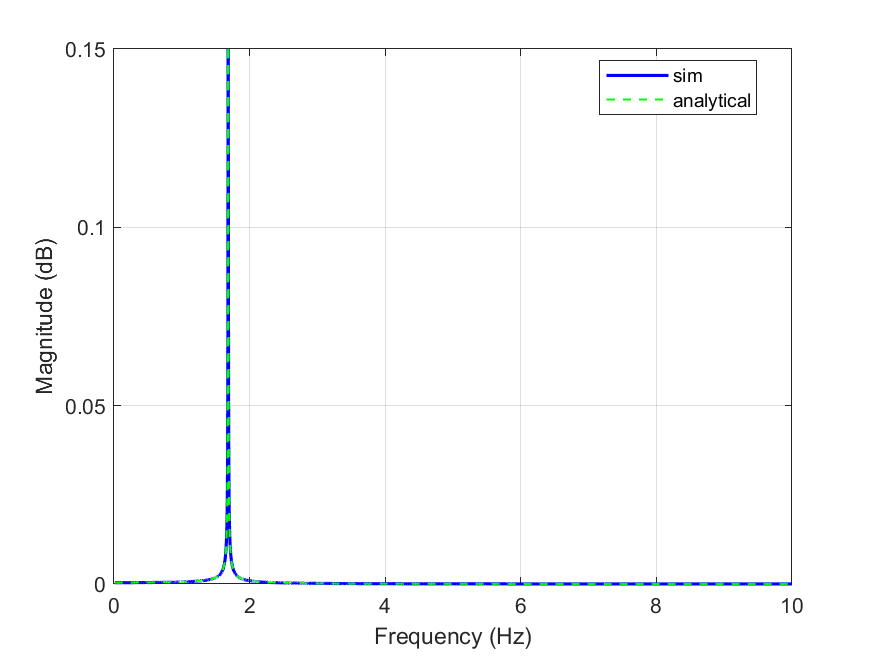
\includegraphics[width=0.8\textwidth]{freq_ampl4.png}
\caption{Сравнение - АЧХ}
\end{figure}

\begin{figure}[ht]
    \centering
    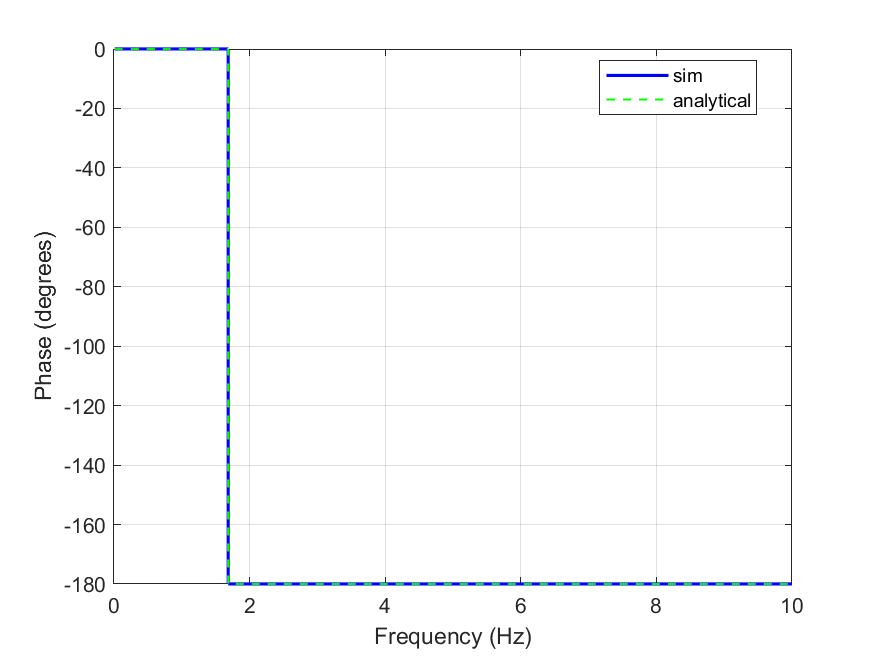
\includegraphics[width=0.8\textwidth]{freq_phase4.png}
  \caption{Сравнение - ФЧХ}
  \end{figure}
\newpage
\begin{figure}[ht]
    \centering
    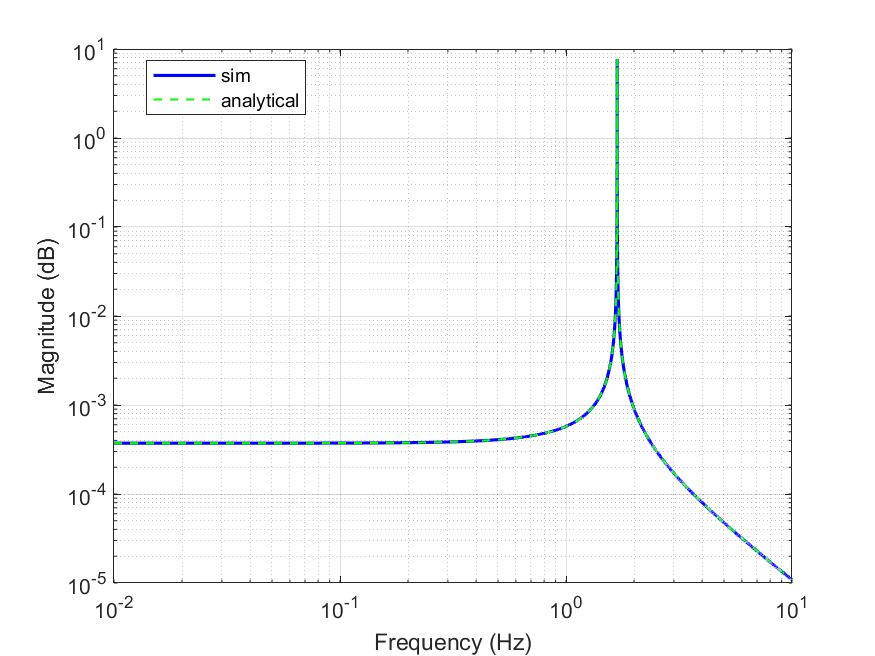
\includegraphics[width=0.8\textwidth]{lfreq_ampl4.png}
  \caption{Сравнение - ЛАЧХ}
  \end{figure}
  
  \begin{figure}[ht]
      \centering
      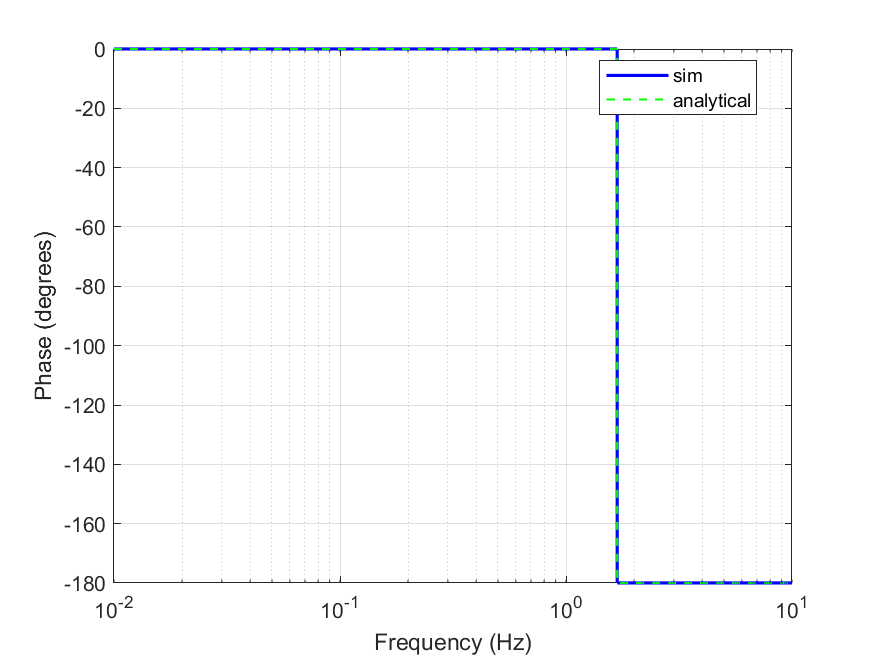
\includegraphics[width=0.8\textwidth]{lfreq_phase4.png}
    \caption{Сравнение - ЛФЧХ}
    \end{figure}

    % \begin{figure}[ht]
    %   \centering
    %   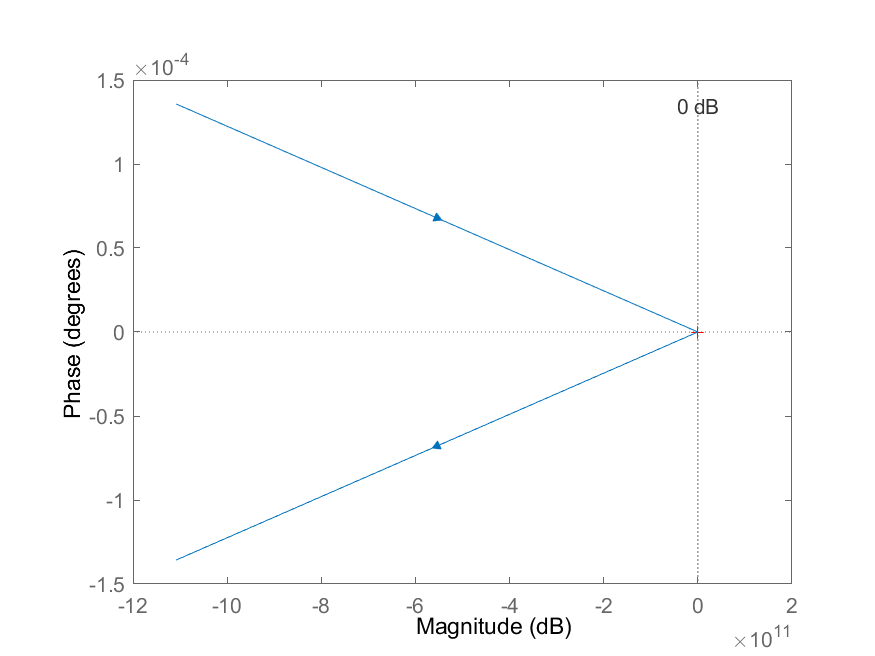
\includegraphics[width=0.8\textwidth]{nyquist4.png}
    % \caption{АФЧХ}
    % \end{figure}
\newpage

\endinput